\documentclass[11pt]{article}
%prepared in AMSLaTeX, under LaTeX2e
\addtolength{\oddsidemargin}{-.75in} 
\addtolength{\evensidemargin}{-.75in}
\addtolength{\topmargin}{-.6in}
\addtolength{\textwidth}{1.4in}
\addtolength{\textheight}{1.3in}

\renewcommand{\baselinestretch}{1.075}

\usepackage{verbatim,fancyvrb}

\usepackage{palatino,amsmath,amssymb,amsthm}

\usepackage{tikz}
\usetikzlibrary{arrows.meta}

\newtheorem*{thm}{Theorem}
\newtheorem*{defn}{Definition}
\newtheorem*{example}{Example}
\newtheorem*{problem}{Problem}
\newtheorem*{remark}{Remark}

\newcommand{\mtt}{\texttt}
\usepackage{alltt,xspace}

%\usepackage[final]{graphicx}

\usepackage[pdftex, colorlinks=true, plainpages=false, linkcolor=blue, citecolor=red, urlcolor=blue]{hyperref}

% macros
\newcommand{\bc}{\mathbf{c}}
\newcommand{\br}{\mathbf{r}}
\newcommand{\bv}{\mathbf{v}}
\newcommand{\bx}{\mathbf{x}}
\newcommand{\by}{\mathbf{y}}

\newcommand{\CC}{\mathbb{C}}
\newcommand{\RR}{\mathbb{R}}
\newcommand{\ZZ}{\mathbb{Z}}

\newcommand{\eps}{\epsilon}
\newcommand{\grad}{\nabla}
\newcommand{\lam}{\lambda}
\newcommand{\lap}{\triangle}

\newcommand{\ip}[2]{\ensuremath{\left<#1,#2\right>}}

%\renewcommand{\det}{\operatorname{det}}
\newcommand{\onull}{\operatorname{null}}
\newcommand{\rank}{\operatorname{rank}}
\newcommand{\range}{\operatorname{range}}

\newcommand{\prob}[1]{\bigskip\noindent\textbf{#1.}\quad }
\newcommand{\exer}[2]{\prob{Exercise #2 in Lecture #1}}

\newcommand{\pts}[1]{(\emph{#1 pts}) }
\newcommand{\epart}[1]{\medskip\noindent\textbf{(#1)}\quad }
\newcommand{\ppart}[1]{\,\textbf{(#1)}\quad }

\newcommand{\Julia}{\textsc{Julia}\xspace}
\newcommand{\Matlab}{\textsc{Matlab}\xspace}
\newcommand{\Octave}{\textsc{Octave}\xspace}
\newcommand{\Python}{\textsc{Python}\xspace}

\DefineVerbatimEnvironment{mVerb}{Verbatim}{numbersep=2mm,
frame=lines,framerule=0.1mm,framesep=2mm,xleftmargin=4mm,fontsize=\footnotesize}

\newcommand{\ema}{\emach}
\newcommand{\emach}{\eps_{\!_{\text{m}}}}

\title{POPDIP: a POsitive-variables \\ Primal-Dual Interior Point optimization method}
\author{Ed Bueler}
\date{\today}

\begin{document}
\maketitle

\begin{abstract}
The algorithm documented here is a modest modification of the Newton-type primal-dual interior point algorithm from \cite[Algorithm 16.1, section 16.7]{GrivaNashSofer2009} and \cite{YamashitaYabe1996}.  It minimizes a smooth nonlinear function subject to the constraints that all the variables are nonnegative, plus linear equality constraints:
\begin{equation}
\begin{matrix}
\text{minimize} \qquad   & f(x) \\
\text{subject to} \qquad & A x = b \\
                         & x \ge 0
\end{matrix} \label{eq:abstractproblem}
\end{equation}

This is a specialized algorithm for nonnegativity constraints $x\ge 0$, and it is not suitable for general inequality constraints of the form ``$g_i(x)\ge 0$,'' and nor is it suitable for general equality constraints ``$g_i(x)=0$.''  However, it can be used as an interior-point method for linear programming in the case where $f(x)=c^\top x$.

These short notes are not research, in the sense that I consider a special case of a well-known algorithm.  Furthermore ``POPDIP'' is a name I made up; it is not in common use.  However, I am interested in this class of methods because local quadratic convergence, seen in unconstrained Newton algorithms, can be proven.  This property is much harder to achieve for constrained problems.
\end{abstract}

\thispagestyle{empty}

\bigskip
\subsection*{Introduction}

Consider first a nonlinear optimization problem with only nonnegativity (informally: positivity) constraints on the variables:
\begin{equation}
\begin{matrix}
\text{minimize} \qquad & f(x) \\
\text{subject to} \qquad & x \ge 0
\end{matrix} \label{eq:posproblem}
\end{equation}
As usual, ``$x\ge 0$'' in \eqref{eq:posproblem} means that each entry of $x\in\RR^n$ is nonnegative.  Here $f:S \to \RR$ is a continuous and smooth function, and the feasible set for \eqref{eq:posproblem} is the convex and closed set $S = \{x\in \RR^n\,:\,x\ge 0\}$ with interior $S^\circ = \{x\in \RR^n\,:\,x > 0\}$.  The next section will address the general problem including linear equality constraints.

One can start the derivation by considering a logarithmic barrier function \cite[section 16.2]{GrivaNashSofer2009}.  Let $\mu>0$ be a (temporarily) fixed constant.  If $x\in S^\circ$ then the following function is well-defined:
\begin{equation}
\beta_\mu(x) = f(x) - \mu \sum_{i=1}^n \ln x_i \label{eq:posbarrierfunction}
\end{equation}
Let $\{e_1,\dots,e_n\}$ be the standard basis of $\RR^n$.  The first-order necessary condition for the \emph{unconstrained} problem of minimizing $\beta_\mu$, namely $\grad \beta_\mu(x)=0$ for $x \in S^\circ$, is
\begin{equation}
\grad f(x) - \mu \sum_{i=1}^n \frac{1}{x_i} e_i = 0 \label{eq:posfirstorderbarrier}
\end{equation}

Conditions \eqref{eq:posfirstorderbarrier} can be reformulated by defining additional variables
    $$\lambda_i = \frac{\mu}{x_i}$$
so that $\lambda\in\RR^n$.  Note that $\lambda>0$ if and only if $x>0$ because $\lambda_i x_i = \mu > 0$.  Then \eqref{eq:posfirstorderbarrier}, plus feasibility for $x$, is equivalent to the following nonlinear system of equations and inequalities:
\begin{align}
\grad f(x) - \lambda &= 0 \label{eq:posfirstordersystem} \\
\lambda_i x_i &= \mu, \qquad i=1,\dots,n \notag \\
x &\ge 0 \notag \\
\lambda &\ge 0 \notag
\end{align}
The feasible set for $x$ and for $\lambda$ is the same, namely $S \subset \RR^n$.  Because of the second condition in \eqref{eq:posfirstordersystem}, both $x$ and $\lambda$ are positive and thus in the interior $S^\circ$.\footnote{By contrast, for the general primal-dual interior point method, specifically Algorithm 16.1 in \cite[section 16.7]{GrivaNashSofer2009}, the feasible set for the primal variable $x$ is different from the dual feasible set for $\lambda$.}

The first condition in \eqref{eq:posfirstordersystem} can be written using a Lagrangian function for \eqref{eq:posproblem}, namely
\begin{equation}
\mathcal{L}(x,\lambda) = f(x) - \sum_{i=1}^n \lambda_i x_i,  \label{eq:poslagrangian}
\end{equation}
in which case it states that $\grad_x \mathcal{L}(x,\lambda)=0$.  In fact, the KKT conditions \cite[sections 14.4, 14.5]{GrivaNashSofer2009} of \eqref{eq:posproblem} are nearly the same as \eqref{eq:posfirstordersystem} but with the second equation replaced by complementarity,
\begin{align}
\grad f(x) - \lambda &= 0 \label{eq:poskkt} \\
\lambda_i x_i &= 0, \qquad i=1,\dots,n \notag \\
x &\ge 0 \notag \\
\lambda &\ge 0 \notag
\end{align}
Thus the barrier method which generated system \eqref{eq:posfirstordersystem} modifies KKT conditions \eqref{eq:poskkt} by changing complementary slackness into a nonzero connection between the primal and dual variables.  (Their product is set to a positive constant.)  System \eqref{eq:posfirstordersystem} describes a solution which is interior to the feasible set and different from the KKT conditions \eqref{eq:poskkt}.

The first condition in \eqref{eq:poskkt} allows $\lambda$ to be eliminated if desired, i.e.~$\lambda = \grad f(x)$.  Writing the conditions without these dual variables gives a \emph{nonlinear complementary problem} (NCP) \cite{FacchineiPang2007},
\begin{equation}
x \ge 0, \qquad \grad f(x) \ge 0, \qquad x_i (\grad f(x))_i = 0.  \label{eq:posncp}
\end{equation}
(Such NCP formulations also appear in problems which are not optimizations, rather variational inequalities \cite{BensonMunson2006,Bueler2016}.)  Thus we may regard POPDIP as solving the $\mu$-modified problem
    $$x \ge 0, \qquad \grad f(x) \ge 0, \qquad x_i (\grad f(x))_i = \mu.$$
However, the method achieves quadratic convergence substantially because it updates both the primal variables $x$ and the dual variables $\lambda$.  Stating the algorithm or the original KKT conditions as an NCP, thereby suppressing the dual variables, is not beneficial.


\subsection*{General problem}

Suppose from now on that $f:\RR^n \to \RR$ is twice continuously-differentiable.  Let $A\in\RR^{m\times n}$, $m\le n$, be a full rank matrix, and suppose $b\in\RR^m$.  The POPDIP algorithm presented in the next section solves the problem
\begin{equation}
\begin{matrix}
\text{minimize} \qquad   & f(x) \\
\text{subject to} \qquad & A x = b \\
                         & x \ge 0
\end{matrix} \label{eq:problem}
\end{equation}

Observe that the constraints are in standard form for linear programming (LP) problems \cite[chapter 4]{GrivaNashSofer2009}.  If $f(x)=c^\top x$ for some fixed $c\in\RR^n$ then \eqref{eq:problem} is an LP problem in standard form, and POPDIP becomes an LP interior point method, though one with no special adaptations to that case; compare e.g.~\cite{ZhangTapiaDennis1992}.

The (primal) feasible set is
\begin{equation}
S = \{Ax=b \text{ and } x\ge 0\} \subset \RR^n.  \label{eq:primalfeasible}
\end{equation}
The iterates $x_k$ from our algorithm will be in the interior,\footnote{In general, $S^0$ is not the topological interior of $S \subset \RR^n$, which is empty if equality constraints apply ($m>0$).} namely in
\begin{equation}
S^o = \{Ax=b \text{ and } x > 0\} \subset \RR^n.  \label{eq:primalinterior}
\end{equation}
We will assume that $S^o$ is nonempty and that an initial iterate in $S^o$ can be found.

Consider the following Lagrangian for \eqref{eq:problem}:
\begin{equation}
\mathcal{L}(x,\tau,\lambda) = f(x) - \tau^\top (Ax - b) - \lambda^\top x, \label{eq:lagrangian}
\end{equation}
for multipliers $\tau\in\RR^m$ and $\lambda\in \RR^n$.  Function \eqref{eq:lagrangian} reduces to \eqref{eq:poslagrangian} if there are $m=0$ linear equality constraints (and $\tau$ is absent).  The first-order necessary conditions, the KKT conditions, for \eqref{eq:problem} are given by $\grad_x\mathcal{L}=0$ and $\grad_\tau\mathcal{L}=0$, plus complementarity for the primal variables $x$ and the dual variables $\lambda$:
\begin{align}
\grad f(x) - A^\top \tau - \lambda &= 0 \label{eq:kkt} \\
-A x + b &= 0 \notag \\
\lambda_i x_i &=0, \qquad i=1,\dots,n \notag \\
x &\ge 0 \notag \\
\lambda &\ge 0 \notag
\end{align}
Conditions \eqref{eq:kkt} reduce to the special case \eqref{eq:poskkt} in the Introduction if there are $m=0$ linear equality constraint.


\subsection*{Algorithm design}

The POPDIP algorithm solves \eqref{eq:problem} by applying a Newton method to a modified form of KKT conditions \eqref{eq:kkt}.  The modification replaces the complementarity condition $\lambda_i x_i = 0$ by the condition
\begin{equation}
\lambda_i x_i = \mu_k, \qquad i=1,\dots,n \notag \\
\end{equation}
for a scalar sequence $\{\mu_k>0\}$ going to zero.  Thus $x_i>0$, so such primal-dual interior point algorithms \cite{NocedalWright2006} compute approximate solutions in the (primal) interior $S^o$.  If the method converges as $\mu_k \to 0$, the limiting values of $x$ and $\lambda$, through never practially achieved because the algorithm is terminated after a finite number of steps, solve the KKT conditions \eqref{eq:kkt}.

Each step of the algorithm is a Newton step for the modified equalities in \eqref{eq:kkt}, namely
\begin{align}
\grad f(x) - A^\top \tau - \lambda &= 0 \label{eq:equalities} \\
-A x + b &= 0 \notag \\
\lambda_i x_i &= \mu_k, \qquad i=1,\dots,n \notag
\end{align}
Because of its third equation, \eqref{eq:equalities} is always a nonlinear system.  However, if $f$ is quadratic or linear then only the modified complementarity condition is nonlinear.

The Newton step computes a search direction in the $x,\tau,\lambda$ variables using the linearization of equations \eqref{eq:equalities}.  (A step will be taken in this search direction, but subject to positivity constraints on $x$ and $\lambda$, via a ratio test \cite[section 3.1]{GrivaNashSofer2009}.)  To describe the step in detail, let $x=x_k+\Delta x$, $\tau=\tau_k+\Delta\tau$ and $\lambda=\lambda_k+\Delta\lambda$.  We assume that the current iterate $(x_k,\tau_k,\lambda_k)$ does not solve \eqref{eq:equalities} exactly.\footnote{Intuitively, an interior-point iteration for \eqref{eq:equalities} sees ``changing equations'' with the iteration count $k$.  As we update the $\mu_k$ value, each new iterate is attempting to solve new equations.  Thus, though the iterates of POPDIP are intended to converge to the solution of KKT problem \eqref{eq:kkt}, they will not converge to a solution of \eqref{eq:equalities} for any $\mu_k>0$.}  The unknowns in the Newton step form the search direction $p=(\Delta x,\Delta\tau,\Delta\lambda)$.  Substituting into \eqref{eq:equalities} and expanding to first order gives
\begin{align}
\grad f(x_k) + \grad^2 f(x_k) \Delta x - A^\top \tau_k - A^\top \Delta \tau - \lambda_k - \Delta \lambda &= 0 \label{eq:prenewtonstep} \\
-A x_k - A \Delta x + b &= 0 \notag \\
(\lambda_k)_i (x_k)_i + (x_k)_i (\Delta\lambda)_i + (\lambda_k)_i (\Delta x)_i &= \mu_k, \qquad i=1,\dots,n \notag
\end{align}

Rearranging \eqref{eq:prenewtonstep} as a vectorized and matrix-block system for the search direction gives
\begin{equation}
\begin{bmatrix}
\grad^2 f(x_k) & -A^\top & -I \\
-A             & 0       & 0  \\
\Lambda_k      & 0       & X_k
\end{bmatrix}
\begin{bmatrix}
\Delta x \\
\Delta \tau \\
\Delta \lambda
\end{bmatrix}
=
\begin{bmatrix}
-\grad f(x_k) + A^\top \tau_k + \lambda_k \\
A x_k - b \\
\mu_k e - \Lambda_k x_k
\end{bmatrix} \label{eq:newtonstep}
\end{equation}
Here $I$ is the $n\times n$ identity matrix, $e=(1,1,\dots,1)^\top$, and we have defined diagonal matrices based on the primal/dual vectors $x_k,\lambda_k\in\RR^n$:
    $$X = \begin{bmatrix} x_1 & & \\ & \ddots & \\ & & x_n \end{bmatrix}, \qquad \Lambda = \begin{bmatrix} \lambda_1 & & \\ & \ddots & \\ & & \lambda_n \end{bmatrix}.$$
Note that $\Lambda_k x_k = X_k \lambda_k$ in this notation.

We will solve system \eqref{eq:newtonstep} using direct linear algebra, namely Matlab's default ``$\backslash$'' linear solver.  Because this direct solver is quite accurate, the residual norm $\|b-A x_k\|$, on the right-hand side of \eqref{eq:newtonstep}, will be very small.  In this sense, system \eqref{eq:newtonstep} imposes the classical null-space requirement on the search direction \cite[chapter 3]{GrivaNashSofer2009}:
\begin{equation}
A \Delta x = 0.  \label{eq:dxnull}
\end{equation}

Use of a direct solver means the implementation is not scalable to large problem sizes $n$.  A scalable implementation should not assemble the full matrix on the left side of \eqref{eq:newtonstep}, as we do here.  Furthermore, it would use an iterative solver which exploits the sparse block structure in \eqref{eq:newtonstep}, including the symmetry of upper-left $2\times 2$ block in the matrix.  Preconditioners \cite{Bueler2021} for the $\grad^2 f(x_k)$ block and the equality-constraint Schur complement \cite[chapters 14]{Bueler2021} should be considered.

Given a solution $p=(\Delta x,\Delta\tau,\Delta\lambda)$ of \eqref{eq:newtonstep}, the update formulas are
\begin{align}
x_{k+1} &= x_k + \alpha_x \Delta x \label{eq:updates} \\
\tau_{k+1} &= \tau_k + \alpha_\tau \Delta \tau \notag \\
\lambda_{k+1} &= \lambda_k + \alpha_\lambda \Delta \lambda \notag
\end{align}
Separate maximum step sizes are used for the three vector variables $x,\tau,\lambda$, though this is not the only choice \cite{YamashitaYabe1996}.  Because the equality constraint equations are linear, the full Newton step $\alpha_\tau=1$ is always used.

The quadratic convergence of a general primal-dual interior point method is proven in subsection 16.7.2 of \cite{GrivaNashSofer2009}.  That method replaces general inequality constraints $g_i(x)\ge 0$ by $g_i(x) - s_i =0$, with slack variables $s_i\ge 0$.  However, in our case this replacement says $x_i-s_i=0$ and $s_i\ge 0$, clearly unneeded.  (It is a meaningless renaming of the existing primal variables $x$.)

Also, the back-tracking globalization of the inequality constraints described in Algorithm 16.1 of \cite{GrivaNashSofer2009}, choosing $\alpha_x$ from $\{1,1/2,1/4,\dots\}$ so that $g_i(x_k + \alpha_x \Delta x) > 0$ for all $i$, is not needed to maintain feasibility of our primal variables because of the linearity of all of the constraint functions in \eqref{eq:problem}.  That is, for constraints $Ax=b$ and $x\ge 0$ a ratio test for $\Delta x$ will guarantee primal feasibility, as in the simplex method \cite[chapter 5]{GrivaNashSofer2009}.

On the other hand, just like in Algorithm 16.1 in \cite{GrivaNashSofer2009}, our optimization algorithm shortens the step in the Newton search direction \emph{only} because of the inequality constraints, and not for the ``usual'' unconstrained minimization line search reasons, for instance to generate sufficient decrease by an Armijo or Wolfe rule \cite[section 11.5]{GrivaNashSofer2009}.  In this sense our method is most suitable for quadratic functions $f(x)$, and it may need additional refinements for more general, especially non-convex, objective functions.  It should be used with caution if the Hessian $\grad^2 f(x)$ varies significantly, or is not positive-definite, during the iteration.

For all of the reasons stated above, POPDIP determines step sizes $\alpha_x,\alpha_\lambda$, for the inequality-constrained primal and dual variables, via a condition of (strict) positivity for $x_{k+1}$ and $\lambda_{k+1}$.  First we choose a value $0<\kappa<1$.  Assuming $x_k\in S^o$, so that $x_k>0$, we require that for all $i$ such that $(\Delta x)_i < 0$,
\begin{equation}
(x_k)_i + \alpha_x (\Delta x)_i \ge (1-\kappa) (x_k)_i > 0 \qquad \iff \qquad \alpha_x \le - \kappa \frac{(x_k)_i}{(\Delta x)_i}. \label{eq:preratio}
\end{equation}
(If $(\Delta x)_i \ge 0$ then $(x_{k+1})_i>0$ automatically.)  Rule \eqref{eq:preratio} should be applied with a preference for $\kappa \approx 1$, so that the inequality constaints are nearly activated, and also with a preference for the Newton step $\alpha_x=1$.  A similar ratio test applies to the dual variables and determines $\alpha_\lambda$.  In summary:
\begin{align}
\alpha_x &= \min_{1\le i\le n} \left\{1, \,-\kappa \frac{(x_k)_i}{(\Delta x)_i} \,:\, (\Delta x)_i < 0\right\}, \label{eq:ratiotests} \\
\alpha_\tau &= 1, \notag \\
\alpha_\lambda &= \min_{1\le i\le n} \left\{1, \,-\kappa \frac{(\lambda_k)_i}{(\Delta \lambda)_i} \,:\, (\Delta \lambda)_i < 0\right\}. \notag
\end{align}
(Compare subsection 16.7.2 in \cite{GrivaNashSofer2009}.)

The optimality test in POPDIP requires that a certain merit function associated to system \eqref{eq:equalities} be smaller than a given tolerance, either in an absolution sense or relative to the initial value of the merit function.  We use the merit function
\begin{equation}
    \nu(x,\tau,\lambda) = \max\{\|\grad f(x)-A^\top \tau - \lambda\|_2,\|b-Ax\|_2,\|\Lambda x\|_2\}.  \label{eq:meritfunction}
\end{equation}
This function is fundamentally the same as in section 16.7 of \cite{GrivaNashSofer2009}, but adapted to our problem, and recall that we expect $\|b-Ax_k\|=0$ to good accuracy after the initial step.  Note that in the limit $\mu_k\to 0$ we have $\nu(x_*,\tau_*,\lambda_*) = 0$ for the exact solution of \eqref{eq:equalities}, but for some $\mu_k > 0$ the exact solution of \eqref{eq:equalities} gives a value $\nu(x_*,\tau_*,\lambda_*)=\sqrt{n}\, \mu_k>0$.

Subsection 16.7.2 of \cite{GrivaNashSofer2009} describes how Algorithm 16.1 should be modified so that, by Theorem 16.17, the algorithm will exhibit the local quadratic convergence.  The Theorem requires a specific update scheme for $\mu_k$, and a specific choice for $\kappa$ in ratio tests \eqref{eq:ratiotests}.  In our case these are equations
\begin{align}
\mu_k &= \min\{\theta \nu(x_k,\tau_k,\lambda_k),\nu(x_k,\tau_k,\lambda_k)^2\}, \label{eq:muupdate} \\
\kappa &= \max\{\bar\kappa,1-\nu(x_k,\tau_k,\lambda_k)\}, \label{eq:kappaformula}
\end{align}
for parameters $0<\theta<1$ and $0<\bar\kappa<1$.  We choose the default values of the parameters as $\theta=0.1$ and $\bar\kappa=0.9$, based on the minimal hints in Example 16.16 in \cite{GrivaNashSofer2009}.

The method by which the initial dual variables are determined (below) is a somewhat ad hoc construction for which I have no reference.  This issue of initialization is discussed in \cite{Gertzetal2004}.


\subsection*{Pseudocode}

We can now present a pseudocode for our algorithm.  The defaults for parameters are $\text{\texttt{rtol}}=10^{-4}$, $\text{\texttt{atol}}=10^{-50}$, $\text{\texttt{maxiters}}=200$, $\theta=0.1$, and $\bar\kappa=0.9$.

\bigskip
\noindent \textsc{Algorithm POPDIP.}
\begin{quote}
\begin{itemize}
\item[\emph{inputs}]  primal initial values (vector) $x_0\in\RR^n$ such that $x_0 > 0$
\item[]  smooth function $f:\RR^n\to\RR$ returning $f(x)$, $\grad f(x)$, and $\grad^2 f(x)$
\item[]  full row rank matrix $A$ of size $m\times n$
\item[]  vector $b\in\RR^m$
\item[\emph{parameters}]  $\text{\texttt{rtol}}>0$
\item[]  $\text{\texttt{atol}}>0$
\item[]  $\text{\texttt{maxiters}}>0$
\item[]  $0<\theta<1$
\item[]  $0<\bar\kappa<1$
\item[\emph{output}]  an estimate $(x_k,\tau_k,\lambda_k)$ of the solution to \eqref{eq:kkt}
\item  determine initial dual variables:
    \renewcommand{\labelenumi}{(\roman{enumi})}
    \begin{enumerate}
    \item $\tau_0 = 0$
    \item $y_0 = \grad f(x_0)$
    \item if $y_0 \le 0$ then $\mu_0=1$; otherwise $\mu_0$ is average of those products $(x_0)_i (y_0)i$ where $(y_0)_i > 0$
    \item $(\lambda_0)_i = \mu_0 / (x_0)_i$ for $i=1,\dots,n$
    \end{enumerate}
\item  for $k=0,1,2,\dots,\text{\texttt{maxiters}}-1$
    \renewcommand{\labelenumi}{(\roman{enumi})}
    \begin{enumerate}
    \item evaluate merit function of KKT conditions \eqref{eq:kkt}:
    $$\nu_k = \max\{\|\grad f(x_k)-A^\top \tau_k - \lambda_k\|_2,\|b-Ax_k\|_2,\|\Lambda_k x_k\|_2\}$$
    \item optimality test: if $\nu_k<\text{\texttt{atol}}$ or $\nu_k<(\text{\texttt{rtol}}) \nu_0$ for $k>0$ then stop
    \item evaluate barrier parameter: $\mu_k = \min\{\theta \nu_k,\nu_k^2\}$
    \item compute Newton step by solving system \eqref{eq:newtonstep} for $(\Delta x,\Delta \tau,\Delta \lambda)$:
    $$\begin{bmatrix}
\grad^2 f(x_k) & -A^\top & -I \\
-A             & 0       & 0  \\
\Lambda_k      & 0       & X_k
\end{bmatrix}
\begin{bmatrix}
\Delta x \\
\Delta \tau \\
\Delta \lambda
\end{bmatrix}
=
\begin{bmatrix}
-\grad f(x_k) + A^\top \tau_k + \lambda_k \\
A x_k - b \\
\mu_k e - \Lambda_k x_k
\end{bmatrix}$$
    \item evaluate ratio test parameter: $\kappa = \max\{\bar\kappa,1-\nu_k\}$
    \item apply ratio tests for step sizes, to keep $x_{k+1},\lambda_{k+1}$ positive:
\begin{align*}
\alpha_x &= \min_{1\le i\le n} \left\{1, \,-\kappa \frac{(x_k)_i}{(\Delta x)_i} \,:\, (\Delta x)_i < 0\right\} \\
\alpha_\tau &= 1 \\
\alpha_\lambda &= \min_{1\le i\le n} \left\{1, \,-\kappa \frac{(\lambda_k)_i}{(\Delta \lambda)_i} \,:\, (\Delta \lambda)_i < 0\right\}
\end{align*}
    \item update to the next iterate:
\begin{align*}
x_{k+1} &= x_k + \alpha_x \Delta x \\
\tau_{k+1} &= x_k + \alpha_\tau \Delta x \\
\lambda_{k+1} &= \lambda_k + \alpha_\lambda \Delta \lambda
\end{align*}
    \end{enumerate}
\end{itemize}
\end{quote}



\subsection*{\Matlab implementation}

The POPDIP algorithm is implemented by a \Matlab code \href{https://github.com/bueler/popdip/blob/main/matlab/popdip.m}{\texttt{popdip.m}}.  If one wants to accept default parameters then the signature is

FIXME $\tau_k$ output too

\medskip
\centerline{\texttt{function [xk,lamk] = popdip(x0,f)}}

\medskip
\noindent For more control the input parameters can be set as follows:

\medskip
\centerline{\texttt{popdip(x0,f,rtol,atol,maxiters,theta,kappabar)}}

\medskip
\noindent The parameters have the default values listed in the last section.  Additional diagnostic outputs can be requested by using more output arguments; if none of them are requested then they are not saved.

\medskip
\centerline{\texttt{[xk,lamk,xklist,lamklist,nuklist,muklist] = popdip(x0,f,\dots)}}

\medskip
\noindent Download the \href{https://github.com/bueler/popdip/blob/main/matlab/popdip.m}{\texttt{popdip.m}} code, this documentation, and the examples shown below from the Github repository
\begin{center}
    \href{https://github.com/bueler/popdip}{\texttt{github.com/bueler/popdip}}
\end{center}


\subsection*{Example 1}

We first try a small 2D test problem in \href{https://github.com/bueler/popdip/blob/main/matlab/small.m}{\texttt{small.m}}:
\begin{equation}
\begin{matrix}
\text{minimize} \qquad & f(x) = \frac{1}{2} (x_1-1)^2 + \frac{1}{2} (x_2+1)^2 \\
\text{subject to} \qquad & x \ge 0
\end{matrix} \label{testoneproblem}
\end{equation}
For this objective function $f$ the unconstrained minimum is the infeasible point $\hat x =(1,-1)^\top$.  A sketch shows that the exact solution of the constrained problem is $x_*=(1,0)^\top$.  Running the code with the given initial iterate $x_0=(2,2)^\top$ and \texttt{tol} $=10^{-14}$, and otherwise using the default parameters in POPDIP, gives
\begin{Verbatim}[fontsize=\small]
>> testpopdip([2 2]',1.0e-14)
  1:    2.000000000000000    2.000000000000000
  2:    1.641421356237309    0.641421356237310
  3:    1.245446520462486    0.245446520462486
  4:    1.069404818969903    0.069404818969903
  5:    1.013447008853577    0.013447008853577
  6:    1.000537794151783    0.000537794151783
  7:    1.000000867357066    0.000000867357066
  8:    1.000000000002257    0.000000000002257
  9:    1.000000000000000    0.000000000000000
\end{Verbatim}
The printed columns are $(x_k)_1$ and $(x_k)_2$.  Note the apparent quadratic, or at least strongly superlinear, convergence.  The iterates $x_k$ are graphed in the following figure.

\bigskip
\begin{center}
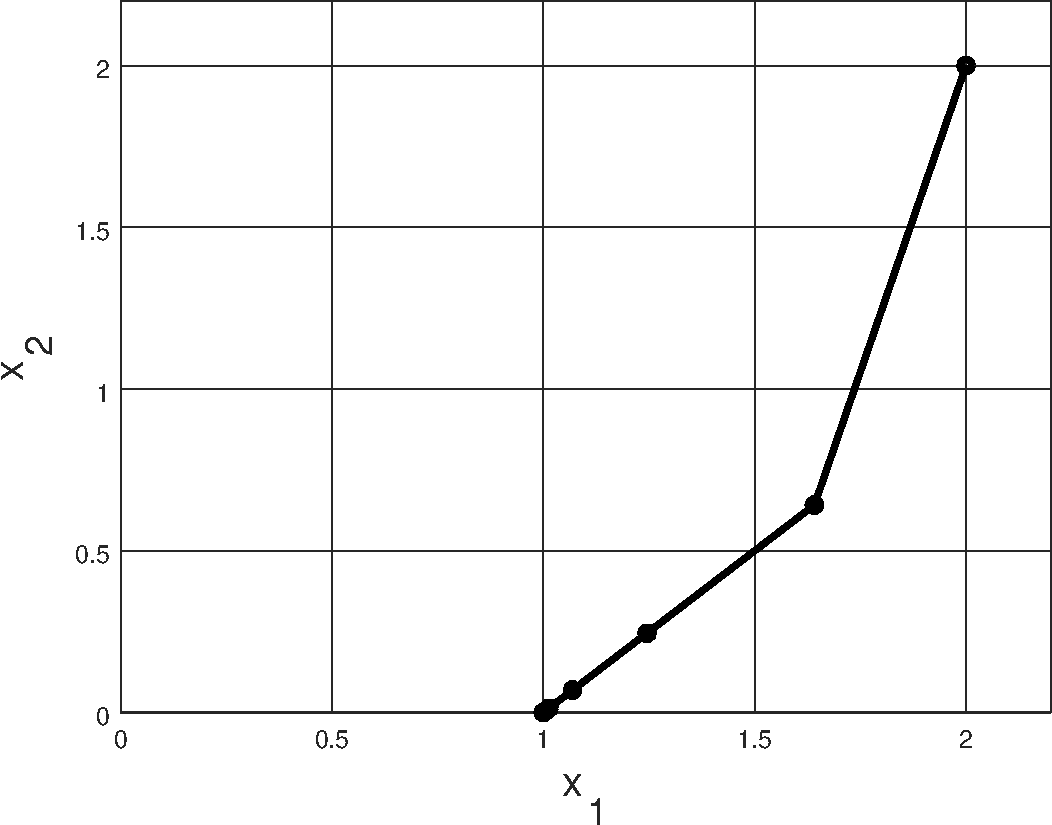
\includegraphics[width=0.6\textwidth]{testpopdip}
\end{center}


\subsection*{Example 2}

FIXME linear programming in 2D


\subsection*{Example 3}

FIXME obstacle problem in 1D: \href{https://github.com/bueler/popdip/blob/main/matlab/obstacle.m}{\texttt{obstacle.m}}

\begin{equation}
    f[u] = \int_0^1 \frac{1}{2} |u'(x)|^2 - q(x) u(x)\,dx \label{obstaclefunctional}
\end{equation}

$\Delta x = 1 / (n+1)$
\begin{equation}
    f(u) = \Delta x \sum_{i=0}^n \left(\frac{1}{2} \left(\frac{u_{i+1}-u_i}{\Delta x}\right)^2 - q(x_{i+1/2}) \frac{u_i + u_{i+1}}{2}\right) \label{obstacleobjective}
\end{equation}
where $u_0=0$ and $u_{n+1}=0$ when they appear

gradient components for $i=1,\dots,n$
\begin{equation}
\grad f(u)_i = \frac{1}{\Delta x} \left\{\begin{matrix}
2 u_1 - u_2 & (i=1) \\
-u_{i-1} + 2 u_i - u_{i+1} & (1<i<n) \\
-u_{n-1} + 2 u_n & (i=n) \\
\end{matrix} \right\} - \frac{\Delta x}{2} (q(x_{i-1/2}) + q(x_{i+1/2}))
\end{equation}

Hessian matrix
\begin{equation}
\grad^2 f(u) = \frac{1}{\Delta x} \begin{bmatrix}
2  & -1 &    &    \\
-1 &  2 & -1 &    \\
   &    & \ddots &\\
   &    & -1 &  2
\end{bmatrix}
\end{equation}

\subsection*{Possible improvements}

FIXME

We may consider possible improvements of our algorithm.  First, in Algorithm 16.1 the computation of the Newton search direction is followed by separate line searches in $x$ and in $\lambda$.  These line searches only maintain nonnegativity and they do not seek sufficient decrease of $f(x)$; they only use ratio tests.  Secondly, equation \eqref{eq:newtonstep} can be symmetrized by multiplying the second half of the equations by $-\Lambda^{-1}$:
\begin{equation}
\begin{bmatrix}
\grad^2 f(x) & - I \\
-I & - \Lambda^{-1} X
\end{bmatrix}
\begin{bmatrix}
\Delta x \\
\Delta \lambda
\end{bmatrix}
=
\begin{bmatrix}
-\grad f(x) + \lambda \\
x - \mu_k \Lambda^{-1} e
\end{bmatrix}
 \label{eq:symmnewtonstep}
\end{equation}

FIXME further simplify into system of $n$ equations for $\lambda$ only

These facts suggests two possible changes:
\begin{enumerate}
\item Back-tracking line search is appropriate as a globalization even for unconstrained optimization.  Thus there must be cases where it is appropriate for problem \eqref{eq:problem} as well.  Once the ratio tests are applied, further back-tracking could be used based on sufficient decrease.  Compare the modified back-tracking line searches in \cite{BensonMunson2006}.
\item One can replace linear system \eqref{eq:newtonstep} with symmetrized system \eqref{eq:symmnewtonstep}.
\end{enumerate}
Determining if these are actual improvements would require testing which we have not done.


%\subsection*{Application to example problem (\texttt{glacier}).}
%FIXME a primal-dual interior point method for a glacier problem appears in \cite{Calvoetal2003}

\medskip

\bibliography{doc}
\bibliographystyle{siam}

\end{document}

